% !TEX root = ./MATH2160.tex
\chapter{Mathematical Programming}\label{chapter:MathematicalProgramming}

Mathematical programming is the subject of locating optimal solutions of problems or systems when they are formulated mathematically. Many important problems in science and engineering take the shape of a mathematical program. We will investigate a few algorithms for nonlinear programming and the simplex algorithm for linear programming.

\section{Nonlinear Programming}

Let $f:\R^n\to\R$, and let $g_i:\R^n\to\R$ and $h_j:\R^n\to\R$. A nonlinear program (NP) is expressed mathematically as:
\mathprog{f(x)}{g_i(x) \le 0,\quad\for\quad i = 1,\ldots,m}{h_j(x) = 0,\quad\for\quad j = 1,\ldots,p}{NP:standardform}

Of course, any maximization problem may be converted into a minimization problem with a sign change, and this may also be used to reformulate constraint equations.

While numerous algorithms\footnote{Some of these algorithms are even derived from the theory of Lagrange multipliers; methods which use Lagrange multipliers as relaxed constraints that iteratively tighten are known as penalty and barrier methods.} have been designed to take advantage of special structure, we will only look at two such algorithms that are applicable in the case of an unconstrained NP. In this section, we will focus solely on the NP:
\begin{align}
\min_{x\in\R^2} f(x) & := e^{\sin(50x_1)} + \sin(60e^{x_2}) + \sin(70\sin(x_1))\nonumber\\
&\quad + \sin(\sin(80x_2)) - \sin(10(x_1+x_2)) + (x_1^2 + x_2^2)/4,\label{eq:SIAM100DigitChallenge}
\end{align}
which appears as Problem $4$ in ``The SIAM $100$-Digit Challenge''~\cite{Bornemann-Laurie-Wagon-Waldvogel-04}.

The first step any mathematician should take when faced with a NP is to obtain realistic bounds on the minimum and its location. For the function~\eqref{eq:SIAM100DigitChallenge}, on a global scale $f$ is dominated by the quadratic term $(x_1^2+x_2^2)/4$, since the values of the first five terms are all bounded in the intervals $[e^{-1},e]$, $[-1,1]$, $[-1,1]$, $[-\sin1,\sin1]$, and $[-1,1]$, respectively. Thus the overall graph of $f$ resembles a familiar paraboloid, depicted in Figure~\ref{figure:MathProgf} (a). A closer look, however, reveals that the trigonometric and exponential terms introduce significant complexity to the fine structure of the function. A contour plot is depicted on a zoomed-in square in Figure~\ref{figure:MathProgf} (b), showing the $2720$ critical points of $f$ inside the square $[-1,1]^2$.

\begin{figure}[htbp]
\begin{center}
\begin{tabular}{cc}
\hspace*{-0.5cm}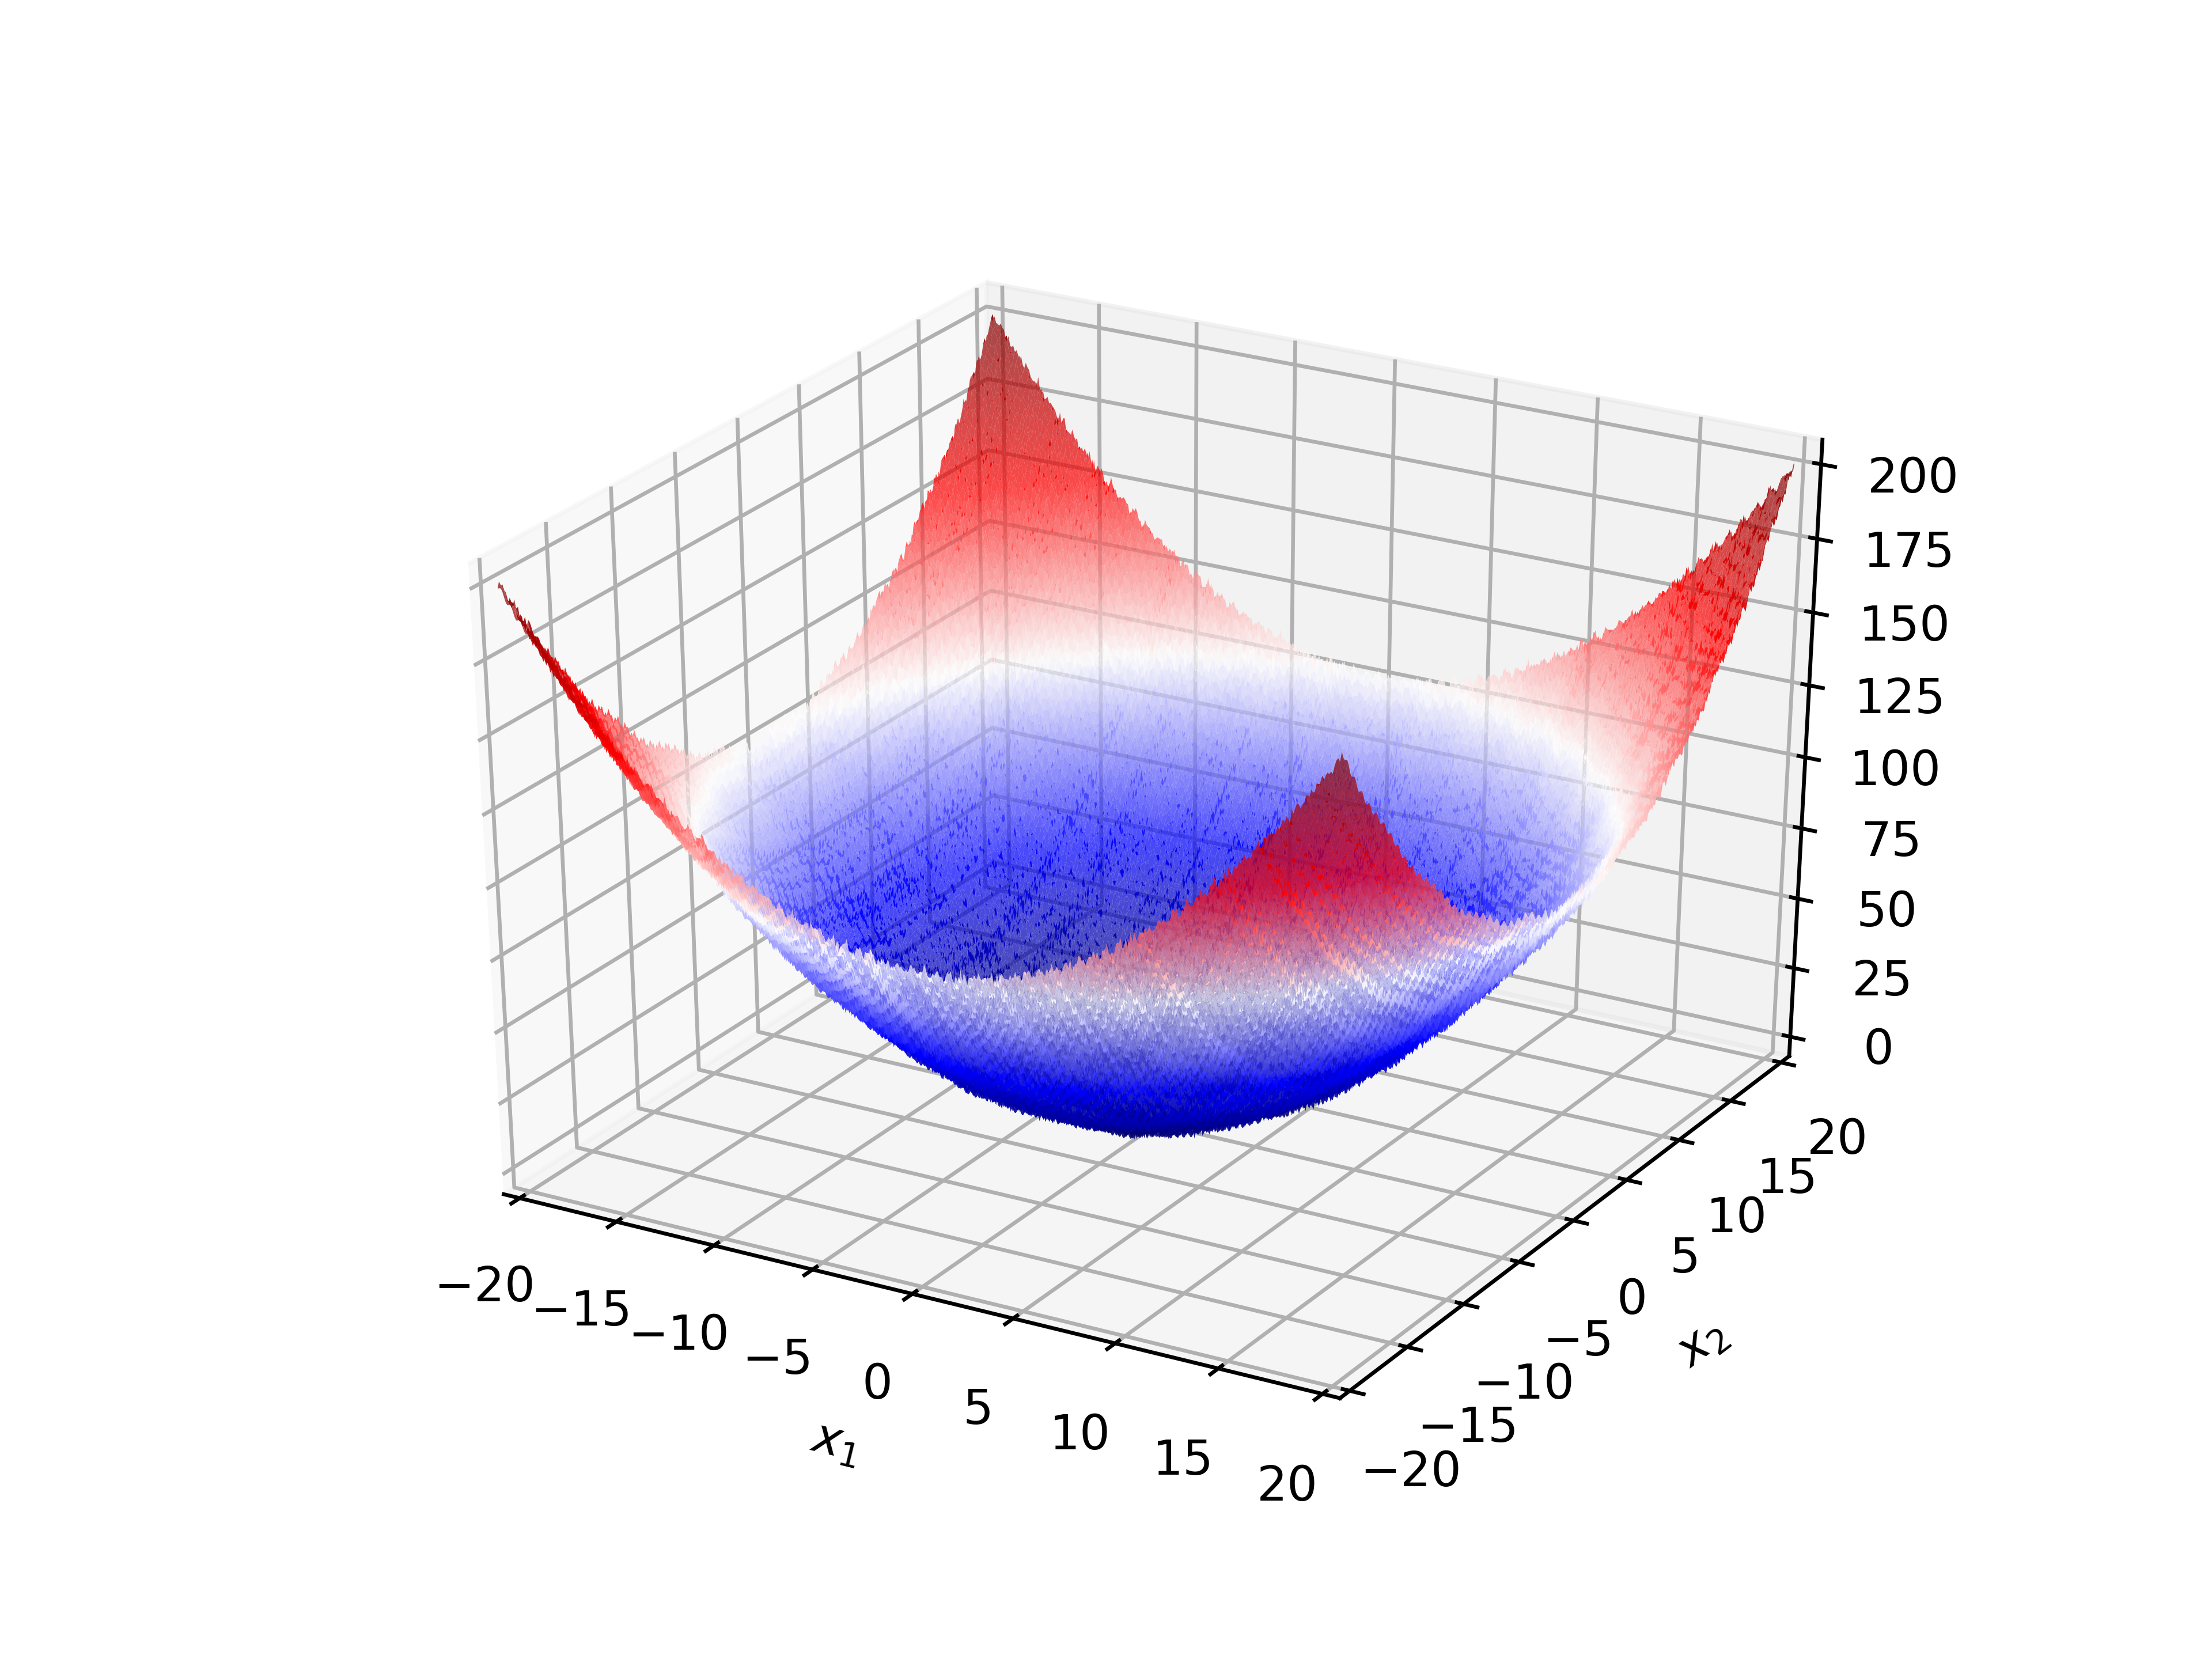
\includegraphics[width=0.525\textwidth]{MathProgf1}&
\hspace*{-0.5cm}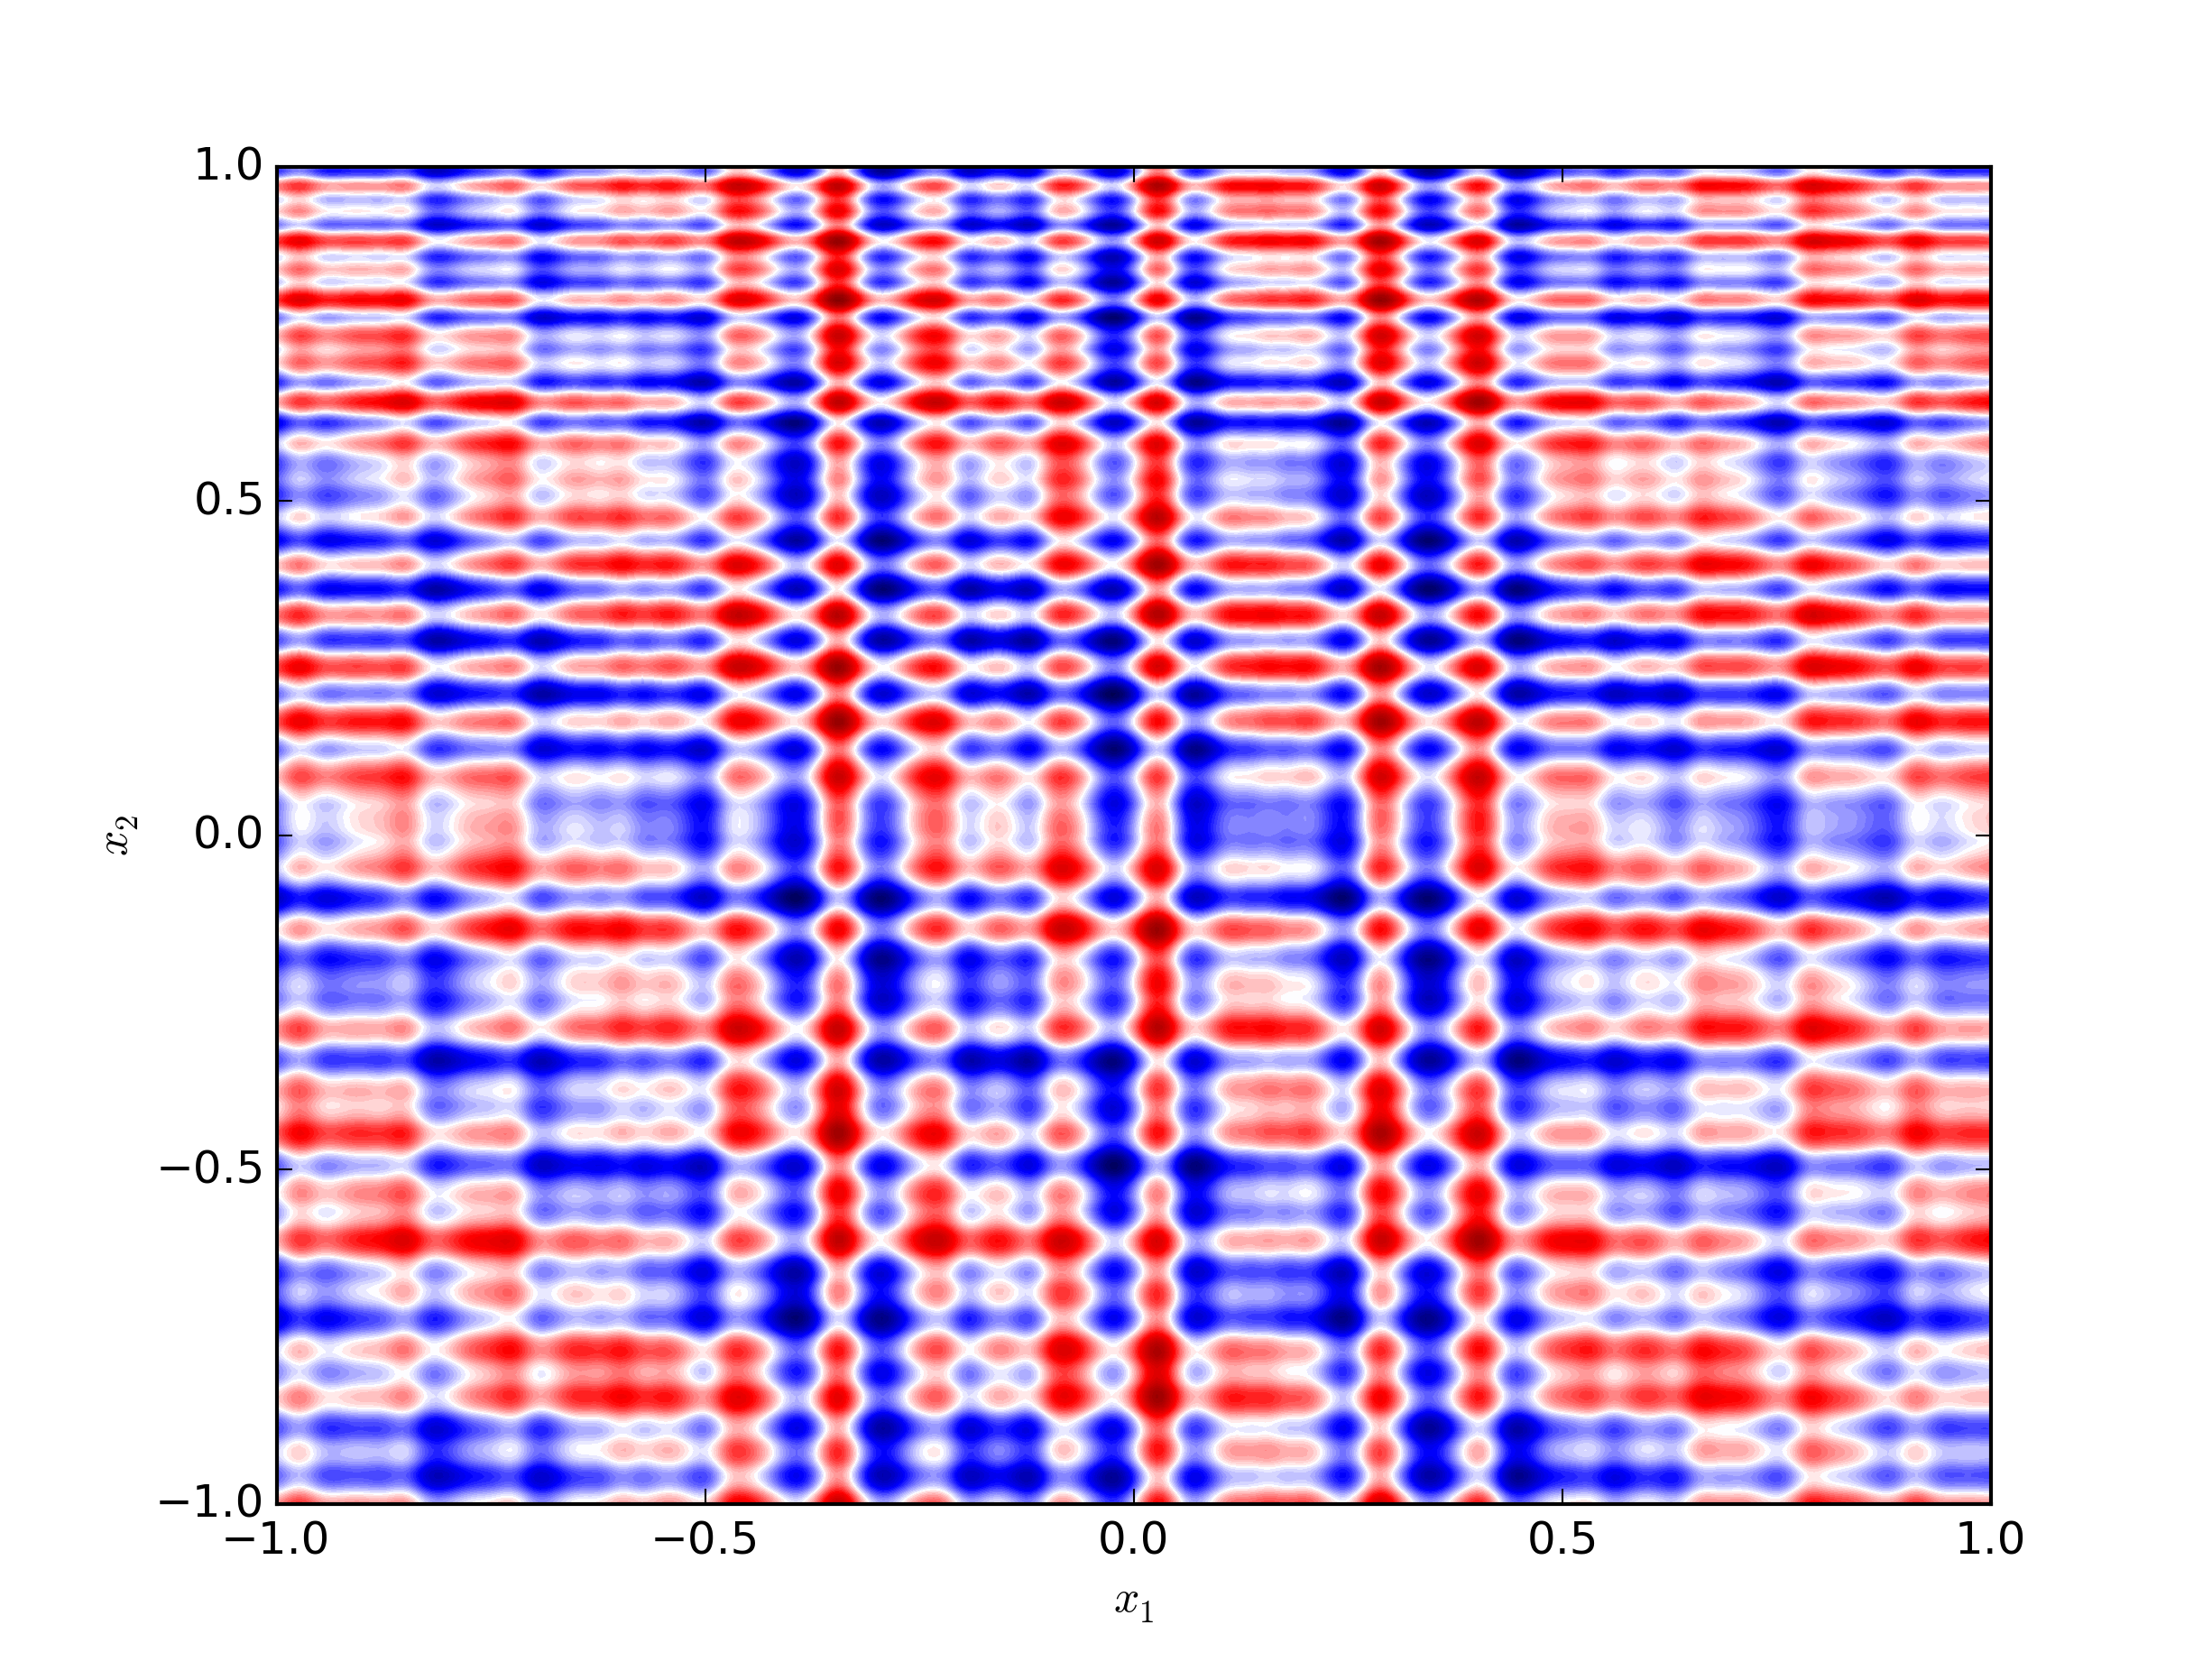
\includegraphics[width=0.525\textwidth]{MathProgf2}\\
(a) & (b)\\
\end{tabular}
\caption{Views of the function~\eqref{eq:SIAM100DigitChallenge}: (a) a surface plot on $[-20,20]^2$ showing the overall paraboloidal shape, and (b) a contour plot on $[-1,1]^2$.}
\label{figure:MathProgf}
\end{center}
\end{figure}

If we evaluate the function at the values of $x_1$ and $x_2$ from $-0.25$ to $0.25$ in steps of $0.01$, we find that the function can be as small as $-3.24$. On the other hand, outside the square $[-1,1]^2$, the function is at least $e^{-1}-1-1-\sin1-1+\frac{1}{4} > -3.23$. Therefore, the global minimum must be inside the square $[-1,1]^2$.

\subsection{Evolutionary Algorithms}

While a grid search can be effective for this particular problem (because the critical points do have a rough lattice structure), it is easy to design a more general search procedure that uses randomness to achieve good coverage of the domain. Several effective algorithms have been derived by abstracting biological processes and theories. Microevolution is a biological theory which describes the dynamics of the gene pool in the members of a species over time. Natural selection and genetic mutation during meiosis are some of the processes that contribute to microevolution. In relation to a NP, for every coordinate $x\in\R^n$, we may associate the {\em fitness value} $f(x)$.

If we begin with a generation of $N_{\rm members}$ random points in a realistic subdomain $D\subset\R^n$, and introduce an additional $N_{\rm members} -1$ points randomly distributed around each of the original $N_{\rm members}$ random points, then we may form a new generation by {\em culling the population} and retaining the $N_{\rm members}$ points-of-best-fit. While we iterate this process, we may use a shrinking scale to define the largest variability of the offspring from their parents.

\begin{algorithm}[Prokaryotic Evolutionary Search]~\\
Inputs: \begin{description} \item[$f(x)$], the objective function;
\item[$D$], the search domain;
\item[$N_{\rm members}$], the number of points in a generation;
\item[$N_{\rm generations}$], the number of generations; and,
\item[$s$], the scaling factor for shrinking the search domain.
\end{description}
Output: an upper bound to the minimum of $f$ in $D$ and its location.
\begin{description}
\item[Step 1:] Initialization:

Let $z$ be the centre of $D$; {\tt parents} = z; and, {\tt fvals = f(z)}.
\item[Step 2:] The main loop:
\begin{verbatim}
for generation = 1:ngenerations
    children = parents
    for p in parents
        append (nmembers-1) random points in D
        centred at p to the children
    end
    fvals = f(children)
    Let parents be the set of nmembers children with lowest fvals
    Shrink D by s
end    
\end{verbatim}
\item[Step 3:] Return:

The smallest value in {\tt fvals} and the corresponding {\tt parent}.
\end{description}
\end{algorithm}

This algorithm may be associated with prokaryotic evolution as the children are strictly descendants from a single parent. If, on the other hand, children may be descendants from two parents, then we obtain a eukaryotic evolutionary search. In the following algorithm, $N_{\rm members}$ children are allowed to be descendants from every pair of parents.

\begin{algorithm}[Eukaryotic Evolutionary Search]~\\
Inputs: \begin{description} \item[$f(x)$], the objective function;
\item[$D$], the search domain;
\item[$N_{\rm members}$], the number of points in a generation; and,
\item[$N_{\rm generations}$], the number of generations.
\end{description}
Output: an upper bound to the minimum of $f$ in $D$ and its location.
\begin{description}
\item[Step 1:] Initialization:

Let {\tt parents} be random points in $D$ and {\tt fvals = f(parents)}.
\item[Step 2:] The main loop:
\begin{verbatim}
for generation = 1:ngenerations
    children = []
    for p in parents, q in parents
        append a random point on the line segment
        in between p and q to the children
    end
    fvals = f(children)
    Let parents be the set of nmembers children with lowest fvals
end    
\end{verbatim}
\item[Step 3:] Return:

The smallest value in {\tt fvals} and the corresponding {\tt parent}.
\end{description}
\end{algorithm}

In Figure~\ref{figure:EvolutionaryAlgorithmError}, an execution of both evolutionary algorithms is depicted for a population with $50$ members, and a scaling factor of $1/2$ for the prokaryotic search. In both (a) and (b), the data represent the discrepancy between the fitness value of every parent in the generation and the global minimum. Clearly, the eukaryotic evolutionary algorithm is able to home in on the global minimum significantly faster than the prokaryotic search. This may be explained as follows: if two parents are equidistant from the global minimum, but on opposite sides (in every coordinate), then we expect a child to appear right over top of the global minimum; on the other hand, no such estimation may be made of prokaryotic evolution.

\begin{figure}[htbp]
\begin{center}
\begin{tabular}{cc}
\hspace*{-0.5cm}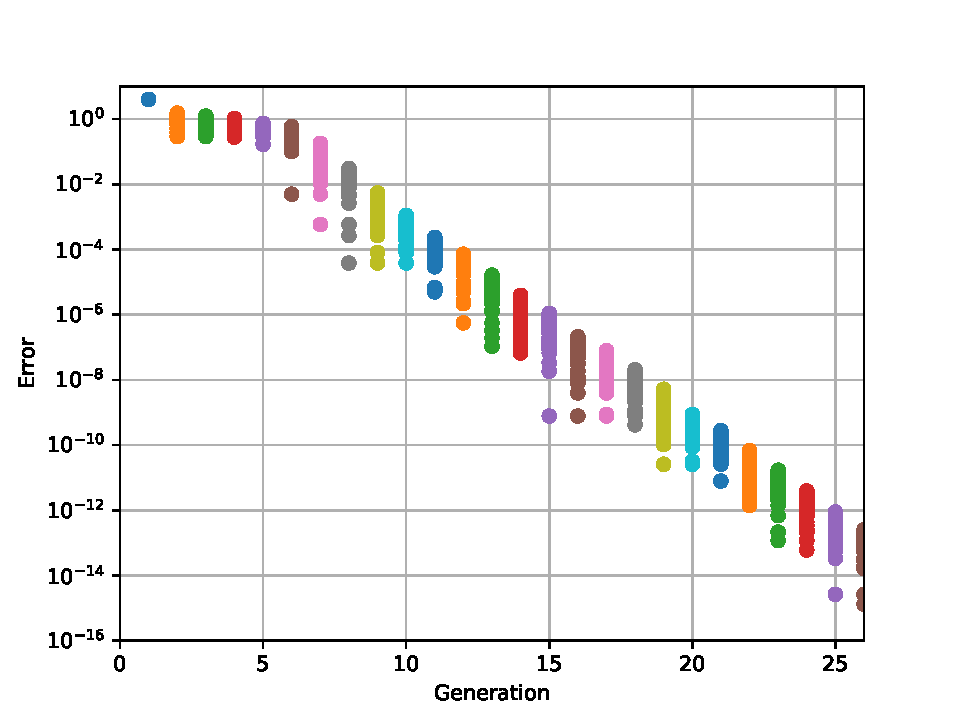
\includegraphics[width=0.525\textwidth]{EvolutionaryAlgorithm1error}&
\hspace*{-0.5cm}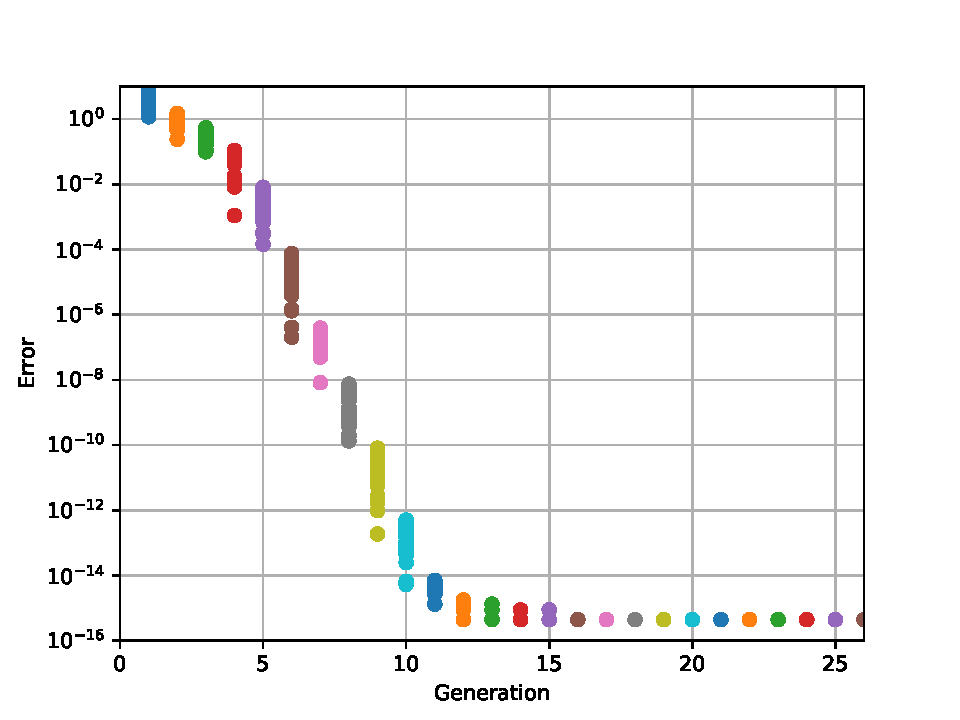
\includegraphics[width=0.525\textwidth]{EvolutionaryAlgorithm2error}\\
(a) & (b)\\
\end{tabular}
\caption{The error of the evolutionary algorithms for the NP~\eqref{eq:SIAM100DigitChallenge} with $50$ members in the population searching through $D=[-1,1]^2$: (a) with prokaryotic search, and (b) with eukaryotic search.}
\label{figure:EvolutionaryAlgorithmError}
\end{center}
\end{figure}

While it is reassuring that the eukaryotic search converges to the global minimum at a faster rate, it is much easier for the algorithm to end up stuck in a local minimizer. Figure~\ref{figure:EvolutionaryAlgorithmProbability} shows the probability of success after $25$ generations of both evolutionary algorithms over $1,000$ iterations. Here, we recognize that the prokaryotic evolutionary search, which supports more random fluctuations throughout the generations, spends more energy ``searching'' through the subdomain $D$ rather than ``settling,'' and is much more likely to succeed with a lower population. This is also reassuring since the earliest living organisms on Earth are thought to be prokaryotes; these organisms had many millions of years to search far and wide for the best (evolutionary) way forward, before eukaryotic search accelerated the process.

\begin{figure}[htbp]
\begin{center}
\begin{tabular}{cc}
\hspace*{-0.5cm}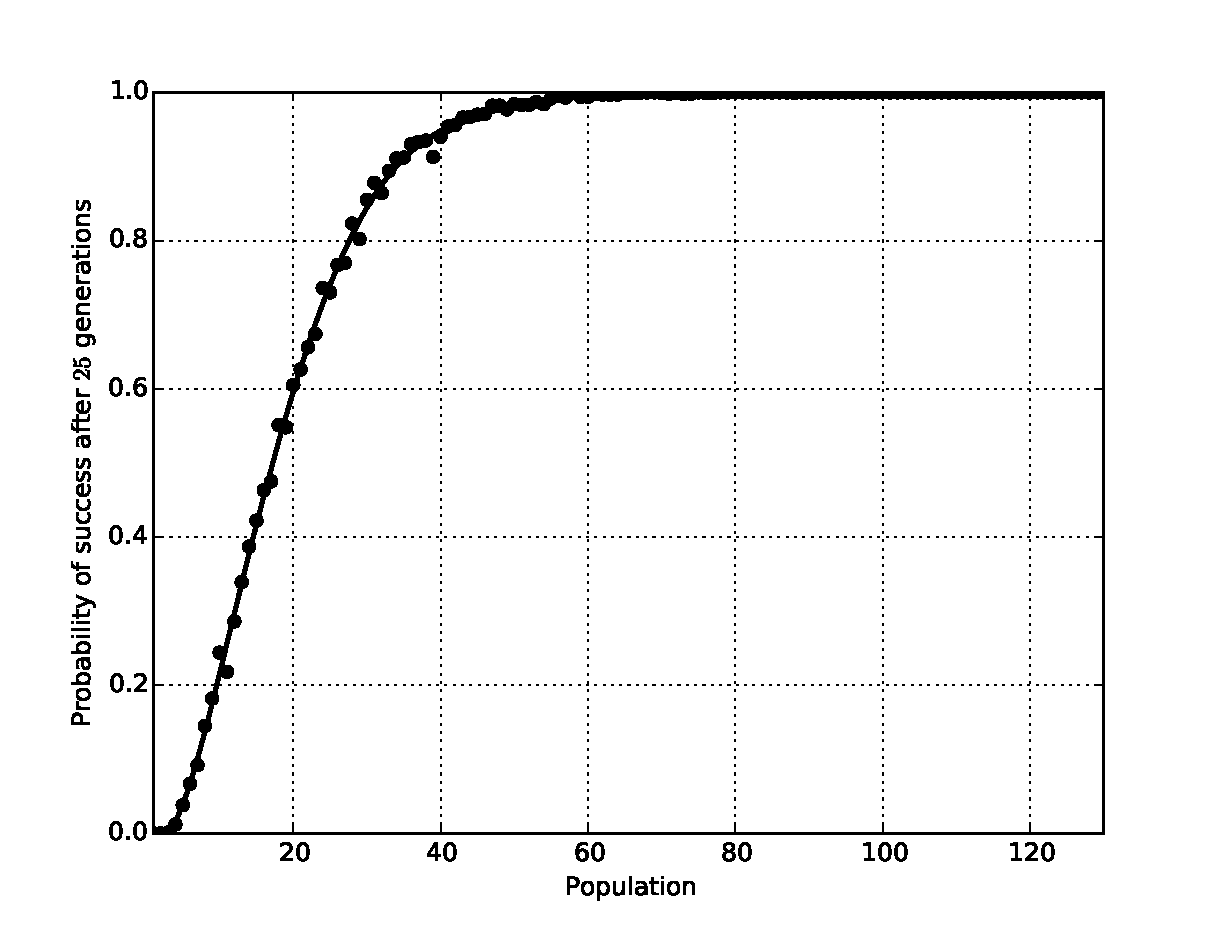
\includegraphics[width=0.525\textwidth]{EvolutionaryAlgorithm1prob}&
\hspace*{-0.5cm}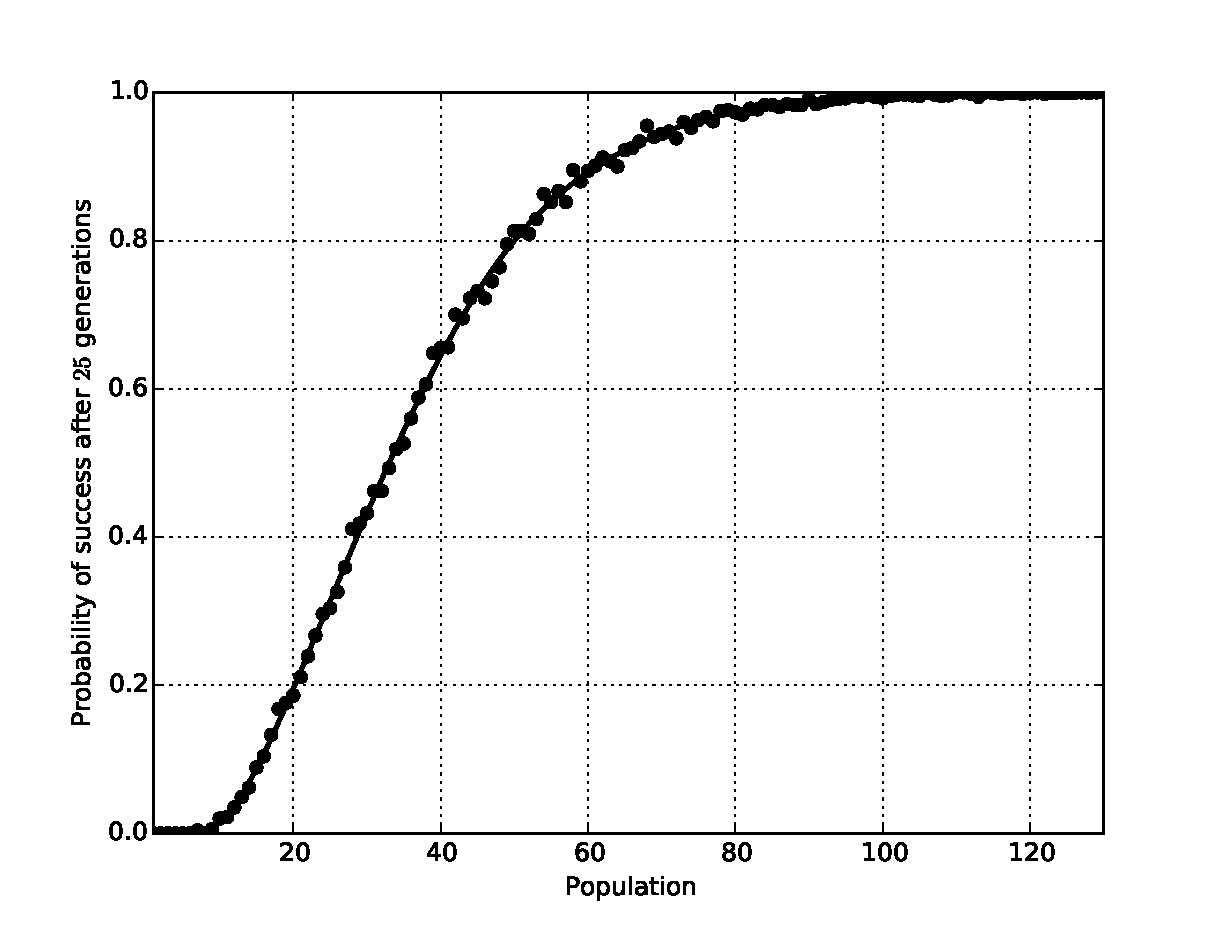
\includegraphics[width=0.525\textwidth]{EvolutionaryAlgorithm2prob}\\
(a) & (b)\\
\end{tabular}
\caption{The probability of success of the evolutionary algorithms over $1,000$ iterations for the NP~\eqref{eq:SIAM100DigitChallenge} searching through $D=[-1,1]^2$: (a) with prokaryotic search, and (b) with eukaryotic search. In both plots, the solid line denotes a degree-$15$ least-squares Chebyshev approximant.}
\label{figure:EvolutionaryAlgorithmProbability}
\end{center}
\end{figure}

Note that both of these algorithms may be adapted to constrained nonlinear programming by rejecting children that do not satisfy the constraints.

\subsection{Quadratic Models}

When we are in striking distance from the global minimizer, we might consider switching to a more efficient algorithm that is able to reproduce extremely high precision results. Recall that a minimizer $x^*$ of a continuously differentiable function $f$ is a critical point:
\[
x^* = \argmin_{x\in\R^n} f(x) \quad \Rightarrow \quad \nabla f(x^*) = 0.
\]
Near a minimizer, we shall approximate a twice continuously differentiable function $f$ by its multivariate Taylor series:
\begin{align*}
f(x+\delta x) & = f(x) + \left[\nabla f(x)\right]^\top \delta x\\
& \quad + \dfrac{1}{2}\delta x^\top \left[\nabla^2 f(x)\right] \delta x + o(\norm{\delta x}^2),\quad {\rm as}\quad \norm{\delta x}\to0.
\end{align*}
To help keep the notation clean, let us introduce $g(x) := \nabla f(x)$ to be the vector of gradients of $f$ and:
\[
H(x) := \nabla^2 f(x) = \begin{bmatrix} \dfrac{\partial^2 f}{\partial x_1^2} & \dfrac{\partial^2 f}{\partial x_1\partial x_2} & \cdots & \dfrac{\partial^2 f}{\partial x_1\partial x_n}\\
\dfrac{\partial^2 f}{\partial x_2\partial x_1} & \dfrac{\partial^2 f}{\partial x_2^2} & \cdots & \dfrac{\partial^2 f}{\partial x_2\partial x_n}\\
\vdots & \vdots & \ddots & \vdots\\
\dfrac{\partial^2 f}{\partial x_n\partial x_1} & \dfrac{\partial^2 f}{\partial x_n\partial x_2} & \cdots & \dfrac{\partial^2 f}{\partial x_n^2}\end{bmatrix},
\]
to be the {\em Hessian}. Then a quadratic approximation to $f$ is:
\[
f(x+\delta x) \approx q(\delta x) = f(x) + g(x)^\top \delta x + \dfrac{1}{2}\delta x^\top H(x) \delta x,
\]
and if we define the vector $\delta x$ by the condition that $\nabla_{\delta x} q(\delta x) = 0$, then we derive Newton's iteration.

\begin{algorithm}[Newton Iteration]~\\
Let $x^{(1)}$ be an initial guess for the global minimizer. For $k\in\N,$
\begin{enumerate}
\item Solve $H(x^{(k)})\delta x^{(k)} = -g(x^{(k)})$, for $\delta x^{(k)}$; and,
\item Set $x^{(k+1)} = x^{(k)} + \delta x^{(k)}$.
\end{enumerate}
\end{algorithm}

The first step in Newton iteration involves the solution of an $n$-by-$n$ system of linear equations. This may be done with a matrix factorization in $\OO(n^3)$ operations\footnote{Quasi-Newton methods are derived by factorizing the matrix $H(x^{(1)})$ once and updating the factorization at every iteration.}. Now that we know how to implement Newton iteration, we may be interested in its convergence properties.

\begin{theorem}
Let $f\in C^2(D)$ and let the Hessian be Lipschitz continuous, i.e. $\abs{H_{i,j}(x) - H_{i,j}(y)} \le K\norm{x-y}$, for some $K>0$, some norm $\norm{\cdot}$, and for $x,y\in D\subset\R^n$. If, for some $k\in\N$, a Newton iterate $x^{(k)}$ is sufficiently close to $x^*\in D$, then Newton's method converges quadratically to $x^*$.
\end{theorem}
\begin{proof}
The Taylor series for each term in $g(x^*)$ is:
\[
0 = g(x^*) = g(x^{(k)}) - H(x^{(k)})e^{(k)} + \OO(\norm{e^{(k)}}^2),
\]
where $e^{(k)} := x^{(k)} - x^*$. Let $x^{(k)}$ be in a neighbourhood of $x^*$ such that $H(x^{(k)})^{-1}$ exists and is bounded above. Such a neighbourhood exists by continuity of $H(x)$. Then, the $k^{\rm th}$ iteration exists, and multiplying through by $H(x^{(k)})^{-1}$ yields:
\[
0 = -\delta x^{(k)} - e^{(k)} + \OO(\norm{e^{(k)}}^2) = -e^{(k+1)} + \OO(\norm{e^{(k)}}^2),
\]
by step 2 of Newton iteration and by definition of $e^{(k+1)}$. Hence by definition of the order notation, there exists a constant $M>0$ such that:
\[
\norm{e^{(k+1)}} \le M\norm{e^{(k)}}^2.
\]
If $x^{(k)}$ is in a neighbourhood for which $\norm{e^{(k)}} < M^{-1}$, then it follows that $\norm{e^{(k+1)}} < \norm{e^{(k)}}$ and by induction, the error contracts and $\displaystyle\lim_{k\to\infty}\norm{e^{(k)}}=0$.
\end{proof}

\section{Linear Programming}

{\em Linear programming} (LP) is a mathematical model for optimizing a linear objective (such as maximum profit or minimum cost) constrained by a list of linear relationships. Linear programming was developed during World War II (independently by the Allies and the Soviet Union) to plan expenditures and returns in order to reduce costs to the army and increase losses to the enemy. It was kept secret until 1947.

The founders of this subject are Leonid Kantorovich, a Russian mathematician who developed LP problems in 1939, George Dantzig, who published the simplex method in 1947, and John von Neumann, who developed the theory of the duality in the same year.

An LP problem in the {\em standard form} is expressed mathematically as:
\mathprog{f(x) := c^\top x}{Ax=b}{x\ge0}{LP:standardform}
where $A\in\R^{m\times n}$ and $m\le n$ (usually $<$). Thus the allowable constraints on the variables are either linear equations or non-negativity bounds. The coefficients $c$ in the linear objective function are often referred to as {\em costs}. An example with four variables ($n=4$) and two equations ($m=2$) is:
\mathprog{x_1 + 2x_2 + 3x_3 + 4x_4}{\begin{array}{rrrrrrrrr} x_1 & + & x_2 & + & x_3 & + & x_4 & = & 1\\
x_1 & & &+ & x_3 & - & 3x_4 & = & \tfrac{1}{2}\end{array}}{x_1\ge0,~x_2\ge0,~x_3\ge0,~x_4\ge0}{LP:example}
More general LP problems can be reduced to standard form without undue difficulty. For example, maximization problems are conveniently re-formulated as $-\hbox{minimize} -f(x)$. Additionally, a general linear inequality $a^\top x \le b$ can be transformed using a slack variable $z$ to the equation $a^\top x + z = b$ and the bound $z\ge 0$. More general bounds $x_i\ge \ell_i$ can be dealt with by a shift of origin, and if no bound exists at all on $x_i$ in the original problem, then the standard form can be reached by introducing non-negative variables $x_i^+$ and $x_i^-$. However, we will concentrate on the solution of problems which are already in the standard form~\eqref{LP:standardform}.

It is important to realize that an LP problem in standard form may have no solution, either because there is no feasible point (the problem is {\em infeasible}), or because $f(x)\to-\infty$ for $x$ in the feasible region (the problem is {\em unbounded}). However, usually there is no difficulty in detecting these situations, and so we will concentrate on the normal case where a solution exists, though it may not be unique.

If~\eqref{LP:standardform} is considered in more detail, it can be seen that if $m=n$, then the equations $Ax=b$ determine a unique solution $x$, and the objective function $c^\top x$ and the bounds $x\ge0$ play no role. In most cases, however, $m<n$ so that the system $Ax=b$ is {\em underdetermined} and $n-m$ degrees of freedom remain. In particular, the system can determine only $m$ variables, given values for the remaining $n-m$ variables. For example, the equations in~\eqref{LP:example-b} can be rearranged as:
\begin{equation}\label{LP:exampleequivalent1}
\begin{array}{rrrrrrr} x_1 & = & \tfrac{1}{2} & - & x_3 & + & 3x_4\\ x_2 & = & \tfrac{1}{2} & & & - & 4x_4\end{array},
\end{equation}
which determines $x_1$ and $x_2$ given values for $x_3$ and $x_4$. Alternatively, the same equations can be rearranged as:
\begin{equation}\label{LP:exampleequivalent2}
\begin{array}{rrrrrrr} x_1 & = & \tfrac{7}{8} & - & \tfrac{3}{4}x_2 & - & x_3\\ x_4 & = & \tfrac{1}{8} & - & \tfrac{1}{4}x_2 &  &\end{array},
\end{equation}
determining $x_1$ and $x_4$ from $x_2$ and $x_3$. It is important to consider what values these remaining $n-m$ variables can take in problems in the standard form. The objective function $c^\top x$ is linear and so contains no curvature which can given rise to a minimizing point. Hence such a point must be created by the conditions $x_i\ge0$ becoming active on the boundary of the feasible region. For example, if~\eqref{LP:exampleequivalent2} is used to eliminate the variables $x_1$ and $x_4$ from the problem~\eqref{LP:example}, then the objective function can be expressed as:
\begin{equation}
c^\top x = x_1 +2x_2 + 3x_3 + 4x_4 = \tfrac{11}{8} + \tfrac{1}{4}x_2 + 2x_3.
\end{equation}
Clearly this function has no minimum value unless the conditions $x_2\ge0$ and $x_3\ge0$ are imposed, in which case the minimum occurs when $x_2=x_3=0$.

To summarize, a solution of an LP problem in standard form always exists at one particular {\em extreme point} or {\em vertex} of the feasible region, with at least $n-m$ variables having {\em zero value}, and the remaining $m$ variables being uniquely determined by the equations $Ax = b$, and taking non-negative values. This result is fundamental to the development of LP methods.

The main difficulty in LP is to find which $n-m$ variables take zero value at the solution and which $m$ variables are not. The first algorithm to solve LP problems is the {\em simplex method}, which tries different sets of possibilities in a systematic way.

\subsection{The Simplex Method}

The simplex method for solving an LP problem in standard form generates a sequence of feasible points $x^{(1)}, x^{(2)},\ldots$ which terminates at a solution. Since there exists a vertex at which the solution occurs, each iterate $x^{(k)}$ is also a vertex. Thus $m$ variables have a non-negative value (usually positive) at $x^{(k)}$ and are referred to as {\em basic variables}, and the remaining $n-m$ variables have zero value and are referred to as {\em nonbasic variables}. In each iteration, the simplex method swaps a basic and nonbasic variable in order to decrease the objective function. The superscript $(k)$ is often omitted for clarity.

In the simplex method, we start by partitioning $A = [A_B | A_N]$ where $A_B$ is non-singular. Partitioning $x^\top = (x_B^\top, x_N^\top)$ conformably and $c^\top = (c_B^\top,c_N^\top)$, then we may write the LP problem~\eqref{LP:standardform} in {\em tableau form}:
\[
\left[\begin{array}{c|c} c^\top & 0\\\hline A & b\end{array}\right] = \left[\begin{array}{cc|c} c_B^\top & c_N^\top & 0\\\hline A_B & A_N & b\end{array}\right].
\]
\begin{example}
The LP problem~\eqref{LP:example} can be reformulated as:
\[
\left[\begin{array}{cccc|c} 1 & 2 & 3 & 4 & 0\\\hline 1 & 1 & 1 & 1 & 1\\ 1 & 0 & 1 & -3 & \tfrac{1}{2}\end{array}\right].
\]
The $2$-by-$2$ sub-block in the lower left is non-singular, $\begin{vmatrix} 1 & 1\\ 1 & 0\end{vmatrix} = -1$, and thus we start by identifying $x_1$ and $x_2$ as the basic variables.
\end{example}
Then, by performing {\em row operations} on the tableau (adding or subtracting multiples of one row from another, or by scaling any row), it is possible to reduce the tableau to the form:
\[
\left[\begin{array}{cc|c} c_B^\top & c_N^\top & 0\\\hline A_B & A_N & b\end{array}\right] \rightarrow \left[\begin{array}{cc|c} 0^\top & \hat{c}_N^\top & -\hat{f}\\\hline I & \hat{A}_N & \hat{b}\end{array}\right],
\]
where $\hat{A}_N = A_B^{-1}A_N$, which represents the {\em reduced form} of the LP problem.
\begin{example}
Performing row operations on the LP problem~\eqref{LP:example}:
\begin{align*}
\begin{array}{c} r_1\leftarrow r_1-r_2\\r_3\leftarrow r_2-r_3\end{array} \Rightarrow \left[\begin{array}{cccc|c} 0 & 1 & 2 & 3 & -1\\\hline 1 & 1 & 1 & 1 & 1\\ 0 & 1 & 0 & 4 & \tfrac{1}{2}\end{array}\right],\\
\begin{array}{c} r_1\leftarrow r_1-r_3\\r_2\leftarrow r_2-r_3\end{array} \Rightarrow \left[\begin{array}{cccc|c} 0 & 0 & 2 & -1 & -\tfrac{3}{2}\\\hline 1 & 0 & 1 & -3 & \tfrac{1}{2}\\ 0 & 1 & 0 & 4 & \tfrac{1}{2}\end{array}\right].
\end{align*}
At this stage, the reduced LP problem is equivalent to:
\mathprog{\tfrac{3}{2} + 2x_3 - x_4}{\begin{array}{rrrrrrrrr} x_1 & & & + & x_3 & - & 3x_4 & = & \tfrac{1}{2}\\
& & x_2 & & & + & 4x_4 & = & \tfrac{1}{2}\end{array}}{x_1\ge0,~x_2\ge0,~x_3\ge0,~x_4\ge0}{LP:examplereduced}
While originally the variables $x_3$ and $x_4$ are the nonbasic variables, and thereby $0$, generally they must be non-negative. Therefore, since the coefficient of $x_4$ is $-1$, a positive perturbation of $x_4$ (less than $1/8$ otherwise $x_2$ would fail its non-negativity constraint!) will decrease the objective.
\end{example}
The next step is to analyze the reduced costs $\hat{c}_N$. If the current vertex is optimal, then the reduced costs satisfy the test:
\begin{equation}\label{eq:LPtest}
\hat{c}_N \ge 0.
\end{equation}
If not, then we permute the nonbasic variable associated with the most negative cost:
\[
j = \argmin_{1\le i \le n-m} [\hat{c}_N]_i,
\]
for the basic variable which is forced to violate its non-negativity constraint first. Row operations are again performed to recover the reduced form of the LP problem. The simplex algorithm terminates when all the reduced costs in the final iteration satisfy the test~\eqref{eq:LPtest}.
\begin{example}
In the LP problem~\eqref{LP:example}, $-1$ is the lowest element in the vector of reduced costs. Therefore, we introduce row operations to make a basis vector to then permute with the basic variable $x_2$:
\begin{align*}
\begin{array}{c} r_3\leftarrow \tfrac{1}{4}r_3\\\end{array} \Rightarrow \left[\begin{array}{cccc|c} 0 & 0 & 2 & -1 & -\tfrac{3}{2}\\\hline 1 & 0 & 1 & -3 & \tfrac{1}{2}\\ 0 & \tfrac{1}{4} & 0 & 1 & \tfrac{1}{8}\end{array}\right],\\
\begin{array}{c} r_1\leftarrow r_1+r_3\\r_2\leftarrow r_2+3r_3\end{array} \Rightarrow \left[\begin{array}{cccc|c} 0 & \tfrac{1}{4} & 2 & 0 & -\tfrac{11}{8}\\\hline 1 & \tfrac{3}{4} & 1 & 0 & \tfrac{7}{8}\\ 0 & \tfrac{1}{4} & 0 & 1 & \tfrac{1}{8}\end{array}\right],\\
\begin{array}{c} c_2\leftrightarrow c_4\\\end{array} \Rightarrow \left[\begin{array}{cccc|c} 0 & 0 & 2 & \tfrac{1}{4} & -\tfrac{11}{8}\\\hline 1 & 0 & 1 & \tfrac{3}{4} & \tfrac{7}{8}\\ 0 & 1 & 0 & \tfrac{1}{4} & \tfrac{1}{8}\end{array}\right].
\end{align*}
After one iteration, the reduced costs are all positive, satisfying the test~\eqref{eq:LPtest}, and therefore we know that the nonbasic variables are exactly $0$. Therefore, the solution to the LP problem~\eqref{LP:example} is $\tfrac{11}{8}$, satisfied by:
\[
x_1 = \tfrac{7}{8},~x_2 = 0,~x_3=0,~x_4 = \tfrac{1}{8}.
\]
\end{example}

\begin{remark}
If more than one iteration of the simplex method is required, it may be difficult for you to keep track of the variables after multiple column permutations. Therefore, it is sufficient to ensure that columns of the identity matrix are present {\em somewhere} in the reduced form at each iteration. The simplex algorithm still terminates when all the reduced costs are positive.
\end{remark}

\begin{example}
\mathprog{\begin{array}{rrrrrrrrr} x_1 & + & 3x_2 & + & x_3 & + & 2x_4 & + & x_5\end{array}}{\begin{array}{rrrrrrrrrrr} x_1 & & & + & 2x_3 & & & + & 4x_5 & = & 3\\
& & 2x_2 & & & + & 3x_4 & & & = & 1\\ x_1 & + & x_2 & + & x_3 & & & & & = & 2\\\end{array}}{x_1\ge0,~x_2\ge0,~x_3\ge0,~x_4\ge0,~x_5\ge0}{LP:example2}
In tableau form, the LP problem is:
\[
\left[\begin{array}{ccccc|c} 1 & 3 & 1 & 2 & 1 & 0\\\hline 1 & 0 & 2 & 0 & 4 & 3\\ 0 & 2 & 0 & 3 & 0 & 1\\ 1 & 1 & 1 & 0 & 0 & 2\end{array}\right].
\]
We perform row operations to obtain a reduced form. Note that the lower left $3$-by-$3$ sub-block is non-singular.
\begin{align*}
\begin{array}{c} ~\\r_3 \leftarrow \tfrac{1}{2}r_3\end{array} \Rightarrow \left[\begin{array}{ccccc|c} 1 & 3 & 1 & 2 & 1 & 0\\\hline 1 & 0 & 2 & 0 & 4 & 3\\ 0 & 1 & 0 & \tfrac{3}{2} & 0 & \tfrac{1}{2}\\ 1 & 1 & 1 & 0 & 0 & 2\end{array}\right]\\
\begin{array}{c} r_1 \leftarrow r_1-r_2\\~\\~\\r_4\leftarrow r_2+r_3-r_4\end{array} \Rightarrow \left[\begin{array}{ccccc|c} 0 & 3 & -1 & 2 & -3 & -3\\\hline 1 & 0 & 2 & 0 & 4 & 3\\ 0 & 1 & 0 & \tfrac{3}{2} & 0 & \tfrac{1}{2}\\ 0 & 0 & 1 & \tfrac{3}{2} & 4 & \tfrac{3}{2}\end{array}\right]\\
\begin{array}{c} r_1 \leftarrow r_1-3r_3+r_4\\r_2\leftarrow r_2-2r_4\\~\\~\end{array} \Rightarrow \left[\begin{array}{ccccc|c} 0 & 0 & 0 & \circled{$-{\rm 1}$} & 1 & -3\\\hline 1 & 0 & 0 & -3 & -4 & 0\\ 0 & 1 & 0 & \fbox{$\tfrac{3}{2}$} & 0 & \tfrac{1}{2}\\ 0 & 0 & 1 & \tfrac{3}{2} & 4 & \tfrac{3}{2}\end{array}\right].
\end{align*}
Now in reduced form, we find that the first reduced cost $[\hat{c}_B]_1<0$, circled, so we will be permuting with the nonbasic variable $x_4$. The second row in the tableau shows that $x_1 -3x_4 - 4x_5=0$. Therefore, increasing $x_4$ will not violate the non-negativity of $x_1$. The third row in the tableau shows that $x_2+\tfrac{3}{2}x_4 = \tfrac{1}{2}$, implying that $x_2$ violates the non-negativity constraint when $x_4\ge\tfrac{1}{3}$. On the other hand, the fourth row in the tableau shows that $x_3+\tfrac{3}{2}x_4+4x_5 = \tfrac{3}{2}$, implying that $x_3$ violates the non-negativity constraint when $x_4\ge1$. Thus, by increasing the nonbasic variable $x_4$, the basic variable $x_2$ will violate the non-negativity constraint before $x_3$. Therefore, the pivot is boxed.
\begin{align*}
\begin{array}{c} ~\\r_3 \leftarrow \tfrac{2}{3}r_3\end{array} \Rightarrow \left[\begin{array}{ccccc|c} 0 & 0 & 0 & -1 & 1 & -3\\\hline 1 & 0 & 0 & -3 & -4 & 0\\ 0 & \tfrac{2}{3} & 0 & 1 & 0 & \tfrac{1}{3}\\ 0 & 0 & 1 & \tfrac{3}{2} & 4 & \tfrac{3}{2}\end{array}\right],\\
\begin{array}{c} r_1\leftarrow r_1+r_3\\r_2\leftarrow r_2 + 3r_3\\~\\r_4\leftarrow r_4-\tfrac{3}{2}r_3\end{array} \Rightarrow \left[\begin{array}{ccccc|c} 0 & \tfrac{2}{3} & 0 & 0 & 1 & -\tfrac{8}{3}\\\hline 1 & 2 & 0 & 0 & -4 & 1\\ 0 & \tfrac{2}{3} & 0 & 1 & 0 & \tfrac{1}{3}\\ 0 & -1 & 1 & 0 & 4 & 1\end{array}\right].
\end{align*}
We have returned the LP problem again to reduced form, but this time the reduced costs are all positive. The minimum of $\tfrac{8}{3}$ is attained at $x = (1,0,1,\tfrac{1}{3},0)^\top$.
\end{example}

It became apparent that the tableau form is inefficient in that it updates the entire tableau $\hat{A}_N$ at each iteration. In fact, all the operations in the simplex method can be carried out with an explicit knowledge of $A_B^{-1}$. Since $A_B^{-1}$ is often smaller than $\hat{A}_N$, the resulting method, known as the {\em revised simplex method}, is usually more efficient. The effect of a basis change is to replace the column $a_p$ by $a_q$ in $A_B^{(k)}$, which can be written as the rank-one change:
\[
A_B^{(k+1)} = A_B^{(k)} + (a_q-a_p)e_p^\top.
\]
By using the Sherman--Morrison formula:
\[
\left(A+uv^\top\right)^{-1} = A^{-1} - \dfrac{A^{-1}uv^\top A^{-1}}{1+v^\top A^{-1}u},
\]
we can update the inverse of $A_B^{(k+1)}$ directly.

For LP problems over hundreds of variables, the Sherman--Morrison formula leads to instabilities due to amplification of rounding errors. Instead, well-conditioned matrix factorizations, such as the $QR$ factorization are employed to ensure stability. The rank-one update can similarly be effected in the $Q$ and $R$ factors. For LP problems over tens of thousands of variables, the sparsity of the matrix $A$ is captured, and a pivoting strategy is used to preserve as much of the original sparsity in the {\em factors} as possible. This is an area of active research.

\section{Problems}

\begin{enumerate}

\item What and where is the global minimum of the function:
\begin{align*}
f(x) & = e^{\sin(50x_1)} + \sin(60e^{x_2})\sin(60x_3) + \sin(70\sin(x_1))\cos(10x_3)\\
& \quad + \sin(\sin(80x_2)) - \sin(10(x_1+x_3)) + (x_1^2+x_2^2+x_3^2)/4~?
\end{align*}

\item Solve the linear program:
\mathprog{\begin{array}{rrrrrrrrrrr} 3x_1 & + & 5x_2 & + & 4x_3 & + & 2x_4 & + & x_5\end{array}}{\begin{array}{rrrrrrrrrrr} x_1 & & & - & 2x_3 & & & + & 4x_5 & = & 1\\
-x_1 & + & 2x_2 & + & 5x_3 & + & 3x_4 & & & = & 2\\ x_1 & & & + & x_3 & + & 2x_4 & & & = & 1\\\end{array}}{x_1\ge0,~x_2\ge0,~x_3\ge0,~x_4\ge0,~x_5\ge0}{LP:problem}

\end{enumerate}